\documentclass[13]{article}
\newtheorem{exer}{Question}
\usepackage[margin=0.5in]{geometry}
\newtheorem{sln}{Solution}
\usepackage{graphicx}
\newtheorem{note}{Note}
\begin{document}
\begin{center}
\LARGE \textbf{German University In Cairo
	\\ SalahEl-Din Ebeed 
	\\ 48-- Mechatronics 
}
\end{center}
\section{Lecture 4}
\begin{exer}
What are Mechanical properties of a material reflect ?
\end{exer}

It reflects its response or deformation due to a certain load or force.
\begin{exer}
What factor to be considered in measuring mechanical properties ?
\end{exer}
Factors to be considered include the nature of the applied load and its
duration, as well as the environmental conditions. It is possible for the
load to be tensile, compressive, or shear, and its magnitude may be constant
with time, or it may fluctuate continuously.  Application time may be only a
fraction of a second, or it may extend over a period of many years. Service
temperature and humidity may also be important factors.
\begin{exer}
The most common mechanical test  ?
\end{exer}
The tension test, where a specimen is put under pure axially oriented stress (axial tension). The machine simply keeps increasing the load while measuring the load vs elongation. 
\begin{exer}
How to normalize the tension test regardless of the dimensions of the specimen and load ?
\end{exer}
We divide the load by the \textbf{initial area}  to get the stress
\[
\sigma = \frac{L}{A_0} 
.\] 
and we divide the elongation by the \textbf{initial length }to have the strain. 
\[
\epsilon = \frac{\Delta L}{L} 
.\] 
So instead of the force-elongation curve we get what is called the stress-strain curve.
\\
\begin{center}
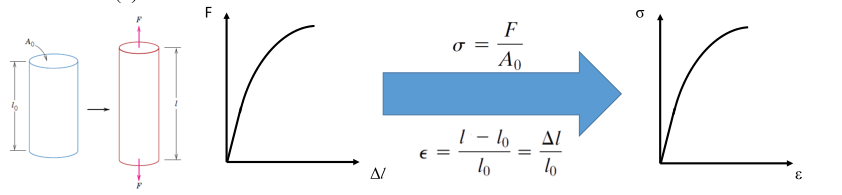
\includegraphics[scale=0.5]{figures/1.png}
\end{center}
\begin{exer}
What do we get from the stress-strain curve ?
\end{exer}
We know the mechanical properties of the material such as: Modulus of Elasticity, Ductility, Resilience, Toughness, UTS, Yield Stress, Allowable stress. (stress or strength)
\begin{exer}
Describe the elastic behaviour ?
\end{exer}
The elastic region or range, is when the tension is at relatively low levels where no bonds are broken, so the material returns to its original shape when The load is removed. Note that the elastic deformation presists only to strains of about 0.005 or (0.5\%).
\begin{exer}
	Where can we find the Yield Stress(Strength) of a material ?
\end{exer}
At the end of the elastic(linear) region.
\begin{exer}
What is young's modulus ? And how do we get it ?
\end{exer}
Young's modulus or the modulus of elasticity (E) is a measure of the material's stiffness. The greater the stiffer the material. \\
We calculate it using the stress-strain graph's elastic region as it is the slope of the linear region. 
\begin{center}
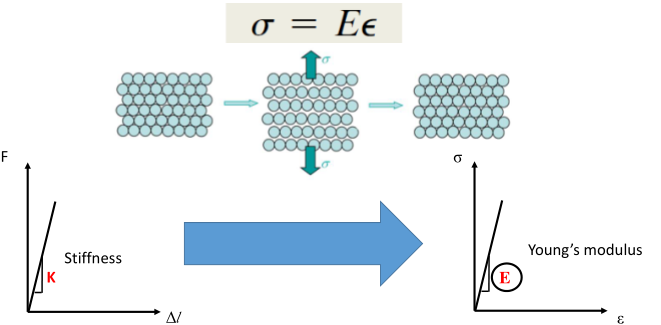
\includegraphics[scale=0.5]{figures/2.png}
\end{center}
\begin{exer}
What are the most stiff elements/materials ?
\end{exer}
Ceramics. They have the highest E.
\begin{exer}
What it the plastic behaviour of a material ?
\end{exer}
After the 0.005 strain (yield strain)  we get to the plastic region, where if the material is deformed in this region it won't get back to its original state or shape. Non-recoverable. In this region there is a slip that happens in the atoms planes.
\begin{center}
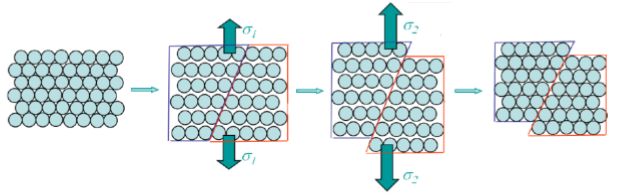
\includegraphics[scale=0.5]{figures/3.png}
\end{center}
\begin{exer}
When does the plastic deformation occur?
\end{exer}
Exactly after the yield stress. $\sigma_y$. At a point P which is called the proportionality limit.
\begin{exer}
	How to find the point P or the yield stress$\sigma_y$ ?
\end{exer}
We go 0.002 (0.2\%) offset, 0.002 of the total deformation (x-axis) and then make a straight line parallel to the elastic region's line. The point we hit is called the P.
\begin{center}
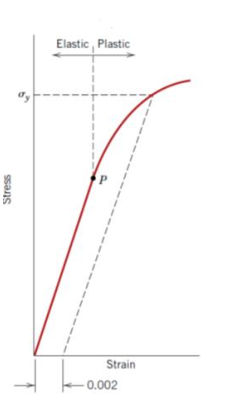
\includegraphics[scale=0.5]{figures/4.png}
\end{center}
\begin{exer}
What is the UTS?
\end{exer}
The ultimate tensile strength, is the stress at the maximum point on the engineering stress-strain curve. After which Necking happens and then the stress decreases as the force decreases and the original area is constant. 
\begin{exer}
What to choose when designing a material to be your safety guideline ?
\end{exer}
We choose the yield strength instead of the ETs and of course divide it by the safety factor in order to get the allowable stress.
\[
	\sigma_{all} = \frac{\sigma_y}{FS} 
.\] 
\begin{exer}
What is Ductility and Brittles ?
\end{exer}
it is a measure of the degree of plastic deformation that has been sustained at fracture . The material that experiences significant plastic deformation until fracture is said to be \textbf{ductile} . (long plastic deformation region).
While the material that exhibits only less than 5\% or no plastic deformation is said to be \textbf{brittle. } 
\begin{exer}
How to calculate Ductility ?
\end{exer}
Well, it is a percent. Percent elongation or percent reduction in area.
\begin{center}
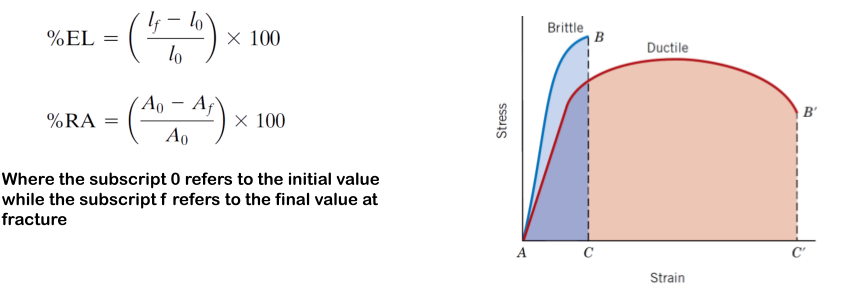
\includegraphics[scale=0.5]{figures/5.png}
\end{center}
\begin{exer}
What is Resilience ?
\end{exer}
it is the capacity of the material to absorb energy while being deformed elastically. And upon unloading this energy is released. It represents the energy per unit volume (Makes sense).   
\begin{exer}
How to measure Resilience ?
\end{exer}
Using the modulus of resilience $U_r$
\[
	U_r = \frac{1}{2} \sigma_y \epsilon_y = \frac{1}{2} \sigma_y (\frac{\sigma_y}{E}) = \frac{\sigma_y^2}{2E} J/m^3 
.\]
\textbf{It is like Spring Energy. The area under the Elastic region Curve
} 
\begin{center}
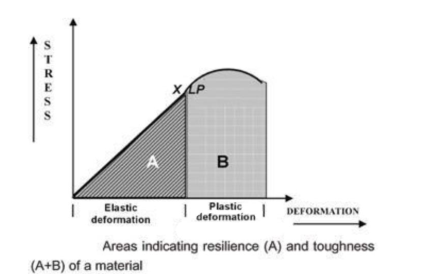
\includegraphics[scale=0.5]{figures/6.png}
\end{center}
\begin{exer}
What is toughness ?
\end{exer}
is the ability of the material to absorb energy and plastically deform before fracturing. Like resilience. 
\begin{exer}
What is the effect of temperature on mechanical properties ?
\end{exer}
We notice from the following graphs that decreasing the temperature decreases the ductility and hence decreases the toughness, but increases the strength of the material.
\begin{center}
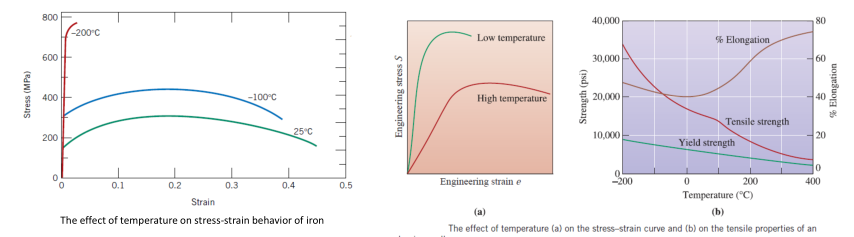
\includegraphics[scale=0.5]{figures/7.png}
\end{center}
\begin{exer}
What is the True stress-strain curve ?
\end{exer}
Instead of the engineering stress-strain curve we have what is called the true stress-strain curve, in which the stress is computed by dividing the current force with the instant's cross sectional area not the original area.
\[
\sigma = \frac{F}{A_i}
.\] 
\begin{exer}
Compare the engineering VS the true stress-strain curve ?
\end{exer}
in the engineering one, after the M point (at which UTS exists), the metal becomes weaker. But this is not true, in face it is increasing in strength. The cross section is decreasing so the stress becomes higher.\\
\begin{exer}
But why does the curve go lower in the engineering one? 
\end{exer}
It is part of the experiment, we choose a certain strain rate to pull the specimen with, So the force needed to pull the specimen decreases with time as the area becomes smaller significantly when necking occurs. The machine decreases the force in order to have the same strain rate.
\begin{exer}
How to calculate the true stress in the curve ?
\end{exer}
\[
\sigma_T = \frac{F}{A_i} 
.\] 
\begin{exer}
How to calculate the true strain ?
\end{exer}
\[
	Elongation = \epsilon_T = \Sigma d\epsilon = \Sigma \frac{dl}{l}=\int \limits_{l_0}^{l} \frac{dl}{l} = ln(l)-ln(l_0) = ln( \frac{l}{l_0})  
.\] 
\begin{exer}
The relationship between the true and engineering stress-strain curves ?
\end{exer}
We can assume that the volume of the specimen is the same (constant) as it deforms \textbf{(but this is before the necking)}  so:
\[
A_0l_0 = Al
.\] 
and Hence:
\[
\sigma_T = \frac{F}{A} = \frac{Fl}{A_0l_0} = \frac{\sigma l}{l_0}
.\] 
\[
l = l_0+\Delta l \\ 
.\] 
\[
\sigma_T = \sigma (1+\frac{\Delta l}{l}) = \sigma (1+ \epsilon)
.\]
and Again
\[
	\epsilon_T = ln(1+ \epsilon)
.\] 
\begin{center}
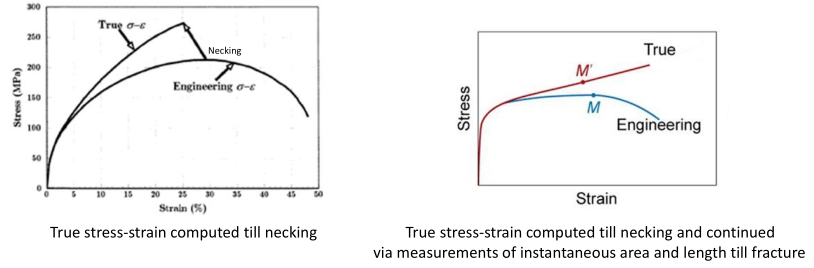
\includegraphics[scale=0.5]{figures/8.png}
\end{center}
\begin{exer}
Define true strain
\end{exer}
The instantaneous elongation per unit length of the specimen.
\begin{exer}
Compare true and engineering stresses and strains.
\end{exer}
The true stress is higher than the Engg. stress, while the true strain is smaller than the Egg. Strain.
\begin{exer}
The relationship between true stress and strain?
\end{exer}
\[
\sigma_T = K \epsilon_T^n
.\] 
This is called the flow stress, K and n are constants and they vary from one metal or alloy to the other. N is called the strain hardening exponent, it is less than 1. 
\begin{exer}
What is the region of the \textbf{flow stress} ?
\end{exer}
it begins after (not from) the yielding point (0.002 or if given) to the necking point (UTS). 





\section{Lecture 5}

\begin{exer}
	What other tests can we use to find mechanical properties ?
\end{exer}
Three point bend test - impact test - hardness test
\begin{exer}
Why normal tensile test cannot easily be done on brittle materials ? 
\end{exer}
\begin{enumerate}
\item it is difficult to prepare and test specimens having the required geometry.
\item it is difficult to grip brittle materials without fracturing them.
\item ceramics fail after only about 0.1\% strain, which necessitates that tensile
specimens be perfectly aligned to avoid the presence of bending stresses
\begin{center}
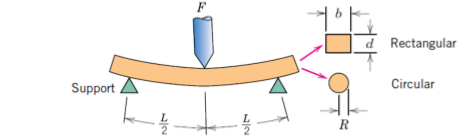
\includegraphics[scale=0.5]{figures/28.png} 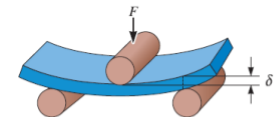
\includegraphics[scale=0.5]{figures/29.png}
\end{center}
\end{enumerate}

\begin{exer}
what is the flexural strength ?
\end{exer}
flexural strength or bend strength or modulus of rupture, is the stress at fracture using the three point bend test. It is an important parameter for brittle materials.
\begin{center}
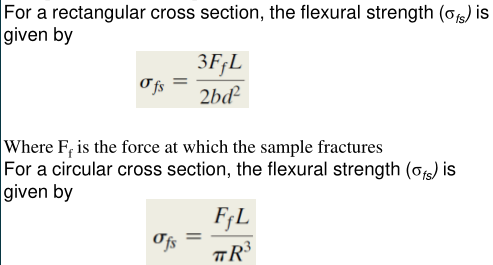
\includegraphics[scale=0.5]{figures/27.png}
\end{center}
\begin{exer}
What does fracture strength depend on ?
\end{exer}
it depends on the specimen size ? Increasing the volume will increase the probability of existence of a crack and thus decrease the flexural strength. 
\begin{exer}
Flexural strength for brittle materials Vs fracture strength from tensile test.
\end{exer}
The fracture strength using the 3point bend test is mush greater than it is measured using tensile test. 
\begin{exer}
But why ?
\end{exer}
This phenomenon may be explained by differences in specimen volume that are
exposed to tensile stresses: The entirety of a tensile specimen is under
tensile stress, whereas only some volume fraction of a flexural specimen is
subjected to tensile stresses—those regions in the vicinity of the specimen
surface opposite to the point of load application .
\begin{exer}
how different the results of 3point test 
\end{exer}
The flexural strength has units of stress. The results of the bend test are
similar to the stress-strain curves; however, the stress is plotted versus
deflection rather than versus strain since we actually care more about
strength rather than ductility. 
\begin{exer}
What happens in the impact test ?
\end{exer}
a material is subjected to a sudden intense blow from a weighted pendulum hammer related from a cocked position at a fixed height, strain rate is extremely rapid ($10^3 s^{-1}$). It measures the amount of absorbed energy till fracture. It is similar to toughness but in high strain rates compared to those with the tensile test.
\begin{center}
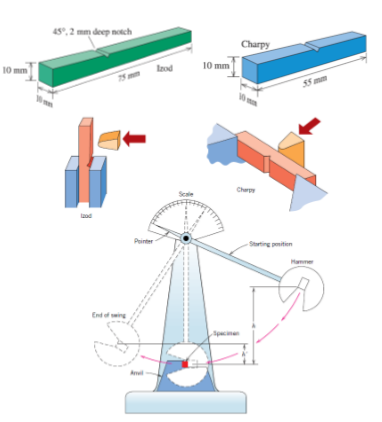
\includegraphics[scale=0.5]{figures/30.png}
\end{center}
the specimen is positioned at the base as shown. Upon release, a knife edge
mounted on the pendulum strikes and fractures the specimen at the notch,
which acts as a point of stress concentration for this high- velocity impact
blow. The pendulum continues its swing, rising to a maximum height h, which
is lower than h. The energy absorption, computed from the difference between
h and h, is a measure of the impact energy.
\[
	E = mg\Delta h = mg(h-h')
.\] 
\begin{exer}
	What else does impact test measure  ?
\end{exer}
besides the absorbed energy, it also determines whether a material experiences a \textbf{ductile-to-brittle transition} with decreasing temperature or not. If so, what is the range of temperatures over which it occurs ?
\begin{center}
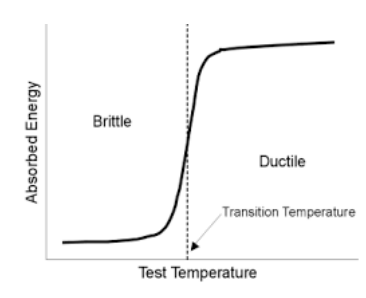
\includegraphics[scale=0.5]{figures/31.png}
\end{center}
\begin{exer}
Ductile vs Brittle material in energy absorption ?
\end{exer}
Ductile materials absorb higher energy until fracture compared to 
brittle materials. Below is  a graph that shows the change in impact 
energy absorbed by carbon steels depending on the carbon content. 
\begin{center}
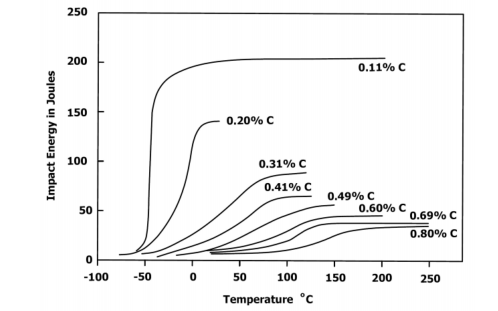
\includegraphics[scale=0.5]{figures/32.png}
\end{center}
\begin{exer}
What is Hardness ?
\end{exer}
Hardness is the resistance of the material to localized plastic deformation (like a small dent, or a scratch depending on context).
\begin{exer}
Describe the Hardness test ?
\end{exer}
In a modern hardness test, a small indenter is forced into the surface of a
material to be tested under controlled conditions of load and rate of
application. The depth or size of the resulting indentation is measured and
related to a hardness number; the softer the material, the larger and deeper
the indentation, and the lower the hardness index number. Most common
hardness tests are the Rockwell, Vicker and Brinell tests. Hardness numbers
are used primarily as a qualitative basis for comparison of materials.
\begin{center}
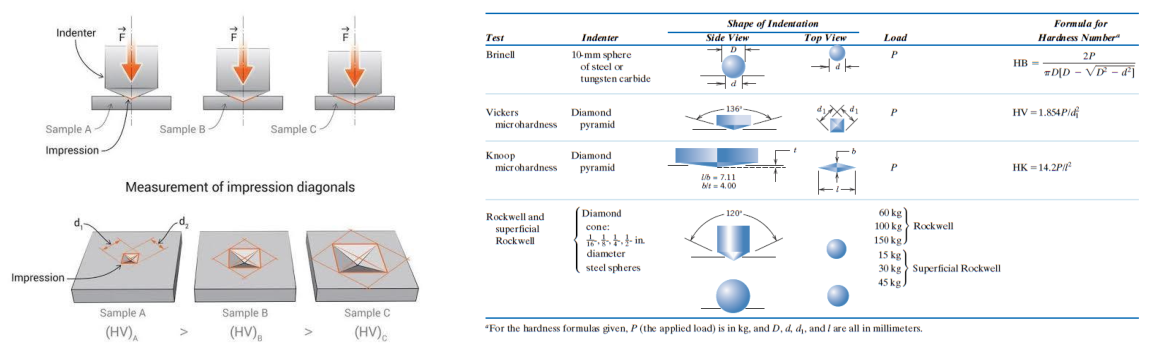
\includegraphics[scale=0.5]{figures/33.png}
\end{center}
\begin{exer}
Hardness and tensile stress/strength ?
\end{exer}
The harder the material the stronger it is. and there is a relation between them. 
\begin{center}
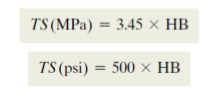
\includegraphics[scale=0.5]{figures/34.png}
\end{center}
\begin{exer}
What are the advantages of Hardness test over other tests ?
\end{exer}
\begin{enumerate}
\item They are simple and inexpensive—typically, no special specimen need be prepared, and the testing apparatus
\item is relatively inexpensive.
The test is non-destructive—the specimen is neither fractured nor excessively deformed; a small indentation is the only deformation.
\item Other mechanical properties often may be estimated from hardness data, such as tensile strength
\end{enumerate}
\begin{exer}
What is fatigue ?
\end{exer}
Fatigue is a form of failure that occurs in structures subjected to dynamic
and fluctuating stresses (e.g., bridges, aircraft, machine components). Under
these circumstances, it is possible for failure to occur at a stress level
considerably lower than the tensile or yield strength for a static load. The
term fatigue is used because this type of failure normally occurs after a
lengthy period of repeated stress or strain cycling. The applied stress
(positive and negative)  may be axial (tension–compression), flexural
(bending), or torsional (twisting) in nature. This is the first
\textbf{time-dependent}  behavior discussed.
\begin{exer}
The fatigue test.
\end{exer}
The most common type of test conducted in a laboratory setting employs a
rotating– bending beam: alternating tension and compression stresses of equal
magnitude are imposed on the specimen as it is simultaneously bent and
rotated. In this case, R = -1.
\begin{center}
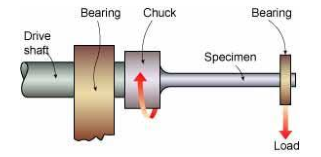
\includegraphics[scale=0.5]{figures/37.png}
\end{center}
Data are plotted as stress versus the logarithm of the number N of cycles to failure for each of the specimens. The S parameter is normally taken as either maximum stress ($\sigma_{max}$) or stress amplitude ($ \sigma_a$) forming what is called the S-N curve.
\begin{center}
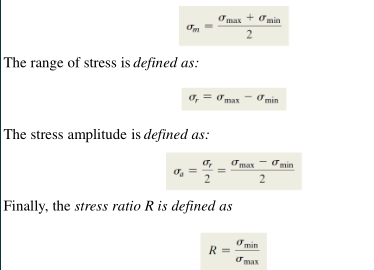
\includegraphics[scale=0.5]{figures/35.png} 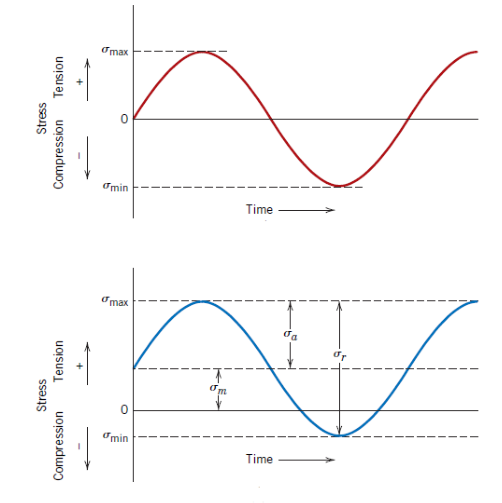
\includegraphics[scale=0.5]{figures/36.png}
\end{center}
\begin{exer}
Relation between number of cycles before fatigue and stress ?
\end{exer}
Two distinct types of S–N behavior are observed for several materials. The higher the magnitude of the stress, the smaller the number of cycles the material is capable of sustaining before failure.
\begin{exer}
What is the fatigue limit/endurance limit ?
\end{exer}
It is the limiting stress, below which fatigue will not occur.
For many steels, fatigue limits range from 35 to 60\% of the tensile strength .

\begin{exer}
	S-N curve for some ferrous(iron-based) and titanium alloys ?
\end{exer}
becomes horizontal at higher N values . 	
\begin{center}
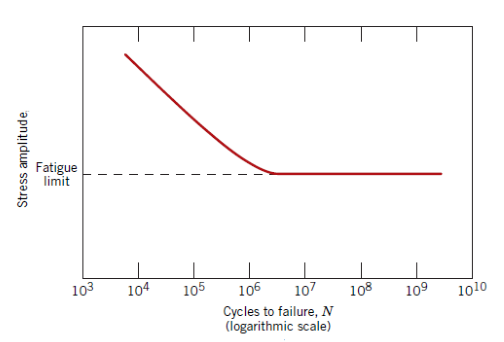
\includegraphics[scale=0.5]{figures/38.png}
\end{center}
\begin{exer}
What is creep property ?
\end{exer}
it is yet another time dependent failure/property of materials. It is the time-dependent and permanent deformation of materials when subjected to a constant load or stress less than the yield strength. For metals, it becomes important for temperatures greater than about 0.4Tm (melting temp). \textbf{Lead (Pb) creeps at room temperature} .
\begin{exer}
What is the creep test ?
\end{exer}
A typical creep test consists of subjecting a specimen to a constant tensile
load or stress while maintaining the temperature constant; deformation or
strain is measured and plotted as a function of elapsed time.
\begin{exer}
What is steady-state creep rate ?	
\end{exer}
it is the slope of the secondary portion of the creep curve. 
\begin{center}
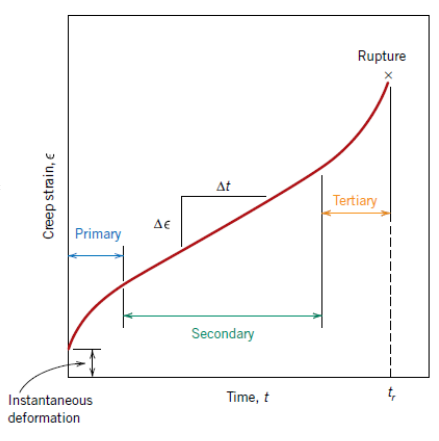
\includegraphics[scale=0.5]{figures/39.png}
\end{center}
\begin{exer}
Relation between creep rate and stress/temp. 
\end{exer}
With either increasing stress or temperature, creep rate increases or rupture lifetime decreases. Time to rupture, or the rupture lifetime $t_r$ is an important parameter. For its determination, creep tests must be conducted to the point of failure; these are termed \textbf{creep rupture tests} .
\begin{exer}
How to improve creep properties ?
\end{exer}
GB sliding is one of the mechanisms responsible for creep, so to overcome GB we do:
\begin{itemize}

\item Conventional casting 
\item Columnar grain
\item Single Crystal 

\end{itemize}



\section{Lecture 6}
\begin{exer}
When does the brittle/ductile behaviour exist ?
\end{exer}
Ones the elastic limit is exceeded, the bonds between the atoms break and the material behaves either in a ductile or brittle manner 
\begin{center}
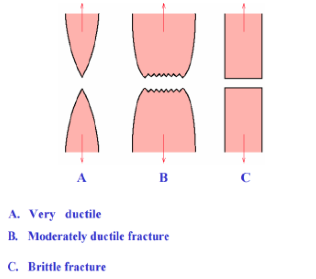
\includegraphics[scale=0.5]{figures/9.png}
\end{center}
\begin{exer}
Explain plastic deformation:
\end{exer}
In ductile materials, the component continue to deform as the force is applied until fracture, this deformation is irreversible.
\begin{exer}
Do brittle material show plastic deformation ?
\end{exer}
Yes, they do, yet this is not significant it is only small amount. As the applied tensile stress breaks the bonds between the atoms and divides the component into two pieces by \textbf{cleavage}. Brittle materials fail in \textbf{tension}  
\begin{exer}
What is ductility ?
\end{exer}
it is basically the motion of dislocations that causes plastic deformation before fracture.
\begin{exer}
What is the cause of plastic deformation ?

\end{exer}
It's basically caused by the slip of one plane of atoms relative to another in \textbf{SHEAR}. 
\begin{center}
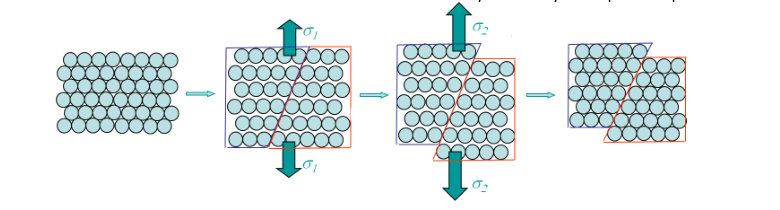
\includegraphics[scale=0.5]{figures/10.png} 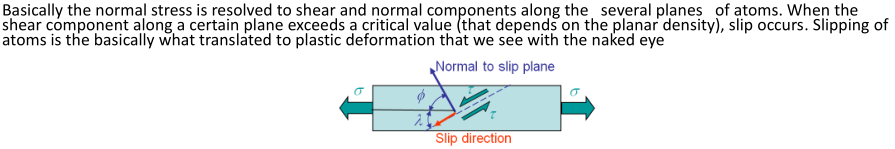
\includegraphics[scale=0.5]{figures/11.png}

\end{center}
\begin{exer}
Explain slip in perfect crystals ?
\end{exer}
it involves breaking and forming of bonds between the atoms while the planes move along one another. This slipping requires so much energy.
\begin{center}
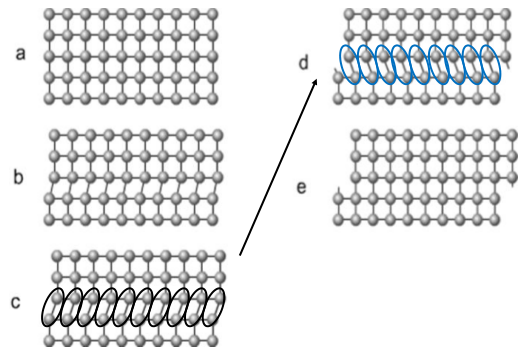
\includegraphics[scale=0.5]{figures/12.png}
This happens in perfect crystals that have no dislocations. (Hypothetical situation)
\end{center}
\begin{exer}
Define Real-life slip ?
\end{exer}
in also involves forming and breaking bonds but it is one at a time. That's why we call it dislocation slip/glide. It makes plastic deformation easier to occur, as the energy needed to break one bond at a time is lower than that needed to break a whole plane of bonds, look at the following figure. 
\begin{center}
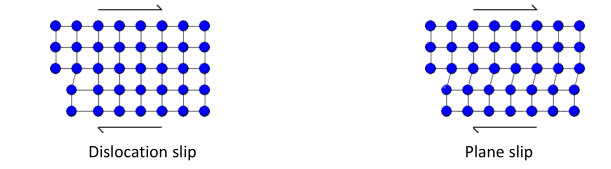
\includegraphics[scale=0.5]{figures/13.png}
\end{center}
\begin{exer}
What are the carriers of plasticity ?
\end{exer}
Dislocations are the carriers of plasticity, because in real life there are no perfect crystals.
\begin{exer}
What happens to the number of dislocations during plastic deformation ?
\end{exer}
The number of dislocation increase dramatically !
\begin{center}
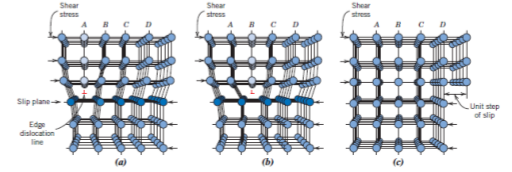
\includegraphics[scale=0.5]{figures/14.png}
\end{center}
\begin{exer}
Define the \textbf{Slip system}  ?
\end{exer}
It's a system that consists of slip plane and a slip direction. The process by which plastic deformation happens itself is called slip.
\begin{center}
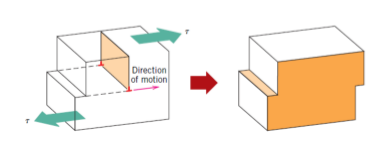
\includegraphics[scale=0.5]{figures/15.png}
\end{center}
\begin{exer}
	What are slip planes and directions ?
\end{exer}
Slip planes are planes which have the highest planar density, and slip direction are those which have the highest linear density. 
\begin{exer}
	Slip occurs first on which type of planes and directions ?
\end{exer}
a smooth plane is the one in which atoms are dense and close together, and thus has higher planar density. So smooth planes are easier to slip.
\begin{exer}
For an FCC material what is the plane that has the highest planar density, or what is the slip plane ?
\end{exer}
it is (111). and the directions along the sides of this plane are the slip directions. 
\begin{exer}
Ductility in polycrystalline materials ?
\end{exer}
Before deformation, the grains are \textbf{equiaxed} or have approximately the same dimensions in all direction. After deformation, grains are elongated in a direction parallel to the load/applied stress direction. (Only that direction). Polycrystalline materials are much stronger than their equivalent single crystalline and thus require higher stresses to initiate slip and yielding. 
\begin{center}
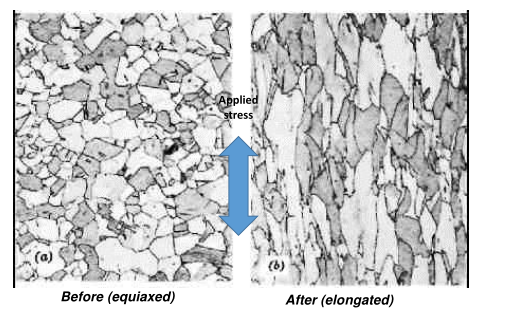
\includegraphics[scale=0.5]{figures/16.png}
\end{center}
\begin{exer}
What is the relation between ductility and bond types in materials ?
\end{exer}
We know that covalent bonds > Ionic > Metallic in Strength. And thus covalent metals such as Silicon and diamond are less ductile than ionic ones such as ceramics .
\begin{exer}
Relation between ductility and strength of a material ?
\end{exer}
The more ductile the material the weaker. And the less ductile the stronger. Inverse relationship.
\begin{exer}
	Why ceramics such as (NaCl) are brittle ?
\end{exer}
because their lattice is consisted of charged ions. Once slip starts and bonds are broken, ions of the same charge come in contact and they don not form any bonds due to repulsion. This leads to brittle fracture since once slip starts to occur, ions repel and fracture happens 
\begin{center}
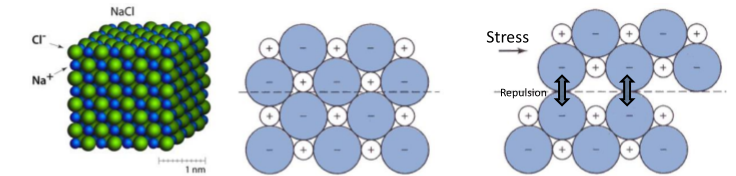
\includegraphics[scale=0.5]{figures/17.png}
\end{center}
\begin{exer}
How to Strengthen one material ?
\end{exer}
Strength (yield and tensile) are related to the ease with which plastic deformation can occur. So reducing the movement of dislocations, will increase the strength and thus decrease the ductility. \textbf{Restricting or hindering dislocation motion renders a material harder and stronger.}  
\begin{exer}
What are the strengthening mechanisms ?
\end{exer}
\begin{itemize}

\item Grain size reduction
\item Solid solution strengthening 
\item Strain hardening

\end{itemize}
\begin{exer}
What happens in grain size reduction technique ?
\end{exer}
We know that grain boundaries are a barrier to the dislocation movement, so in order to decrease dislocation and thus ductility and thus increase strength we increase the grain boundaries by reducing the grain size.
\begin{center}
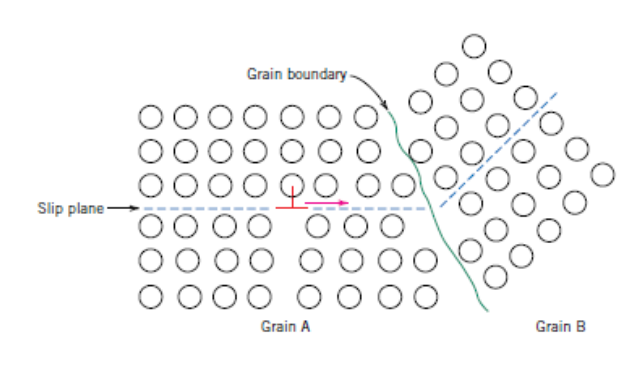
\includegraphics[scale=0.5]{figures/18.png}
\end{center}
Small angle grain boundaries are not very effective in blocking dislocations.
High-angle grain boundaries block slip and increase strength of they material
.
\begin{exer}
How to increase the area of grain boundaries to better impede motion ?
\end{exer}
The finer the grains the larger the area of grain boundaries .
\begin{exer}
What is the Hall-Petch equation ?
\end{exer}
it is the relation that relates yield strength and grain size d.
\[
	\sigma_y = \sigma_0 + k_y(d) - 0.5
.\]
where $\sigma_o$ and k are constants for a particular material, d is the average grain diameter.
\begin{center}
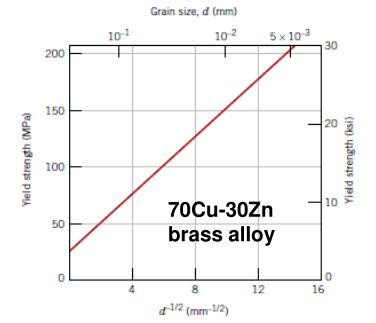
\includegraphics[scale=0.5]{figures/19.png}
\end{center}
\begin{exer}
What are solid solutions ?
\end{exer}
means a commination of two solid or in other words an alloy :). Alloys are usually stringer than pure metals of the solvent. 
\begin{exer}
What happens in Solid-solution strengthening ?
\end{exer}
We use interstitial or substitutional impurities/defects to cause lattice distortion and as a result it hinders the dislocation movement.
\begin{center}
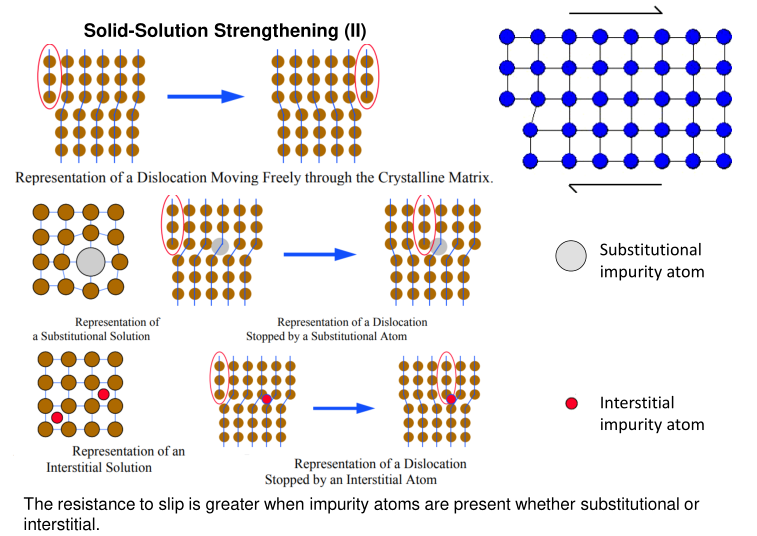
\includegraphics[scale=0.5]{figures/20.png}
\end{center}
\begin{exer}
What makes the solid-solution technique make higher strength ?
\end{exer}
The more the difference between impurity and base material atom sizes (radii), the higher the strengthening. And the higher concentration of the impurity atoms the higher the strength. Look at the following copper materials treated with different impurities. 
\begin{center}
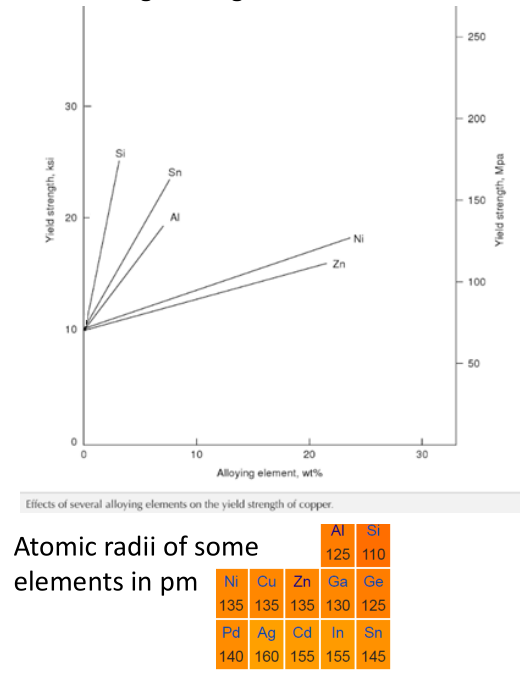
\includegraphics[scale=0.5]{figures/21.png}
\end{center}
The greatest strength happened  with Silicon as the difference in radii is so large. 
\begin{exer}
What happens in the Strain Hardening/Work Hardening/Cold Working?
\end{exer}
Ductile materials become more stronger when they are deformed plastically at temperatures below the melting point. We do this strain hardening in order to increase the dislocation density with applied stress. In this technique we do mechanical forces (like forging) in low temperatures below melting point. Th average distance between dislocations decrease and dislocations start blocking the motion of each other.
\begin{exer}
	Calculate the percent cold work (\%CW). 
\end{exer}
\[
	\% CW = ( \frac{A_0-A_d}{A_0} )*100
.\] 
\%CW is just another measure of the degree of plastic deformation, in addition to strain.
\begin{center}
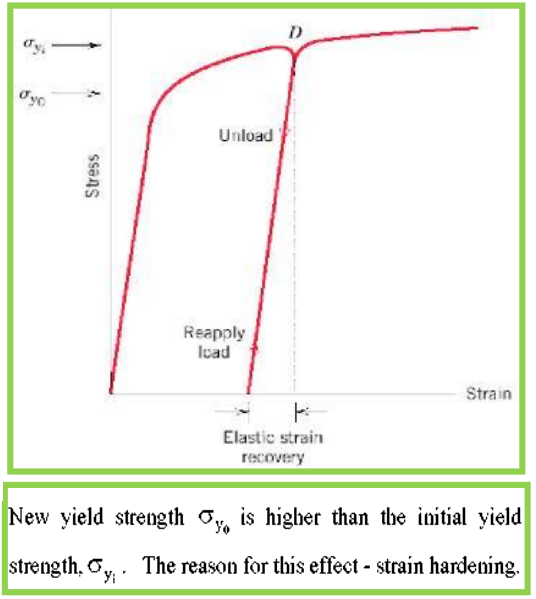
\includegraphics[scale=0.5]{figures/22.png} 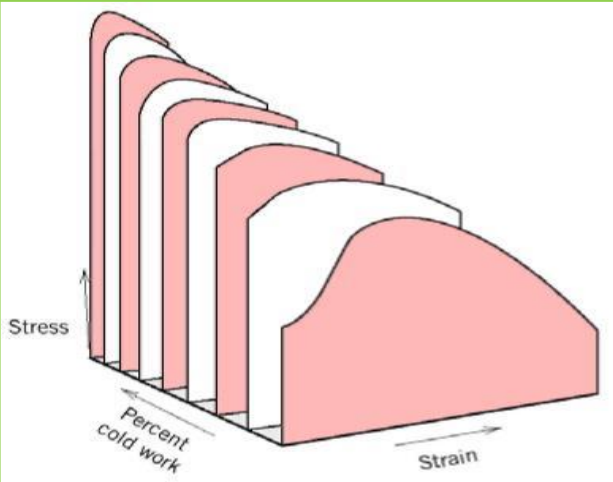
\includegraphics[scale=0.5]{figures/23.png}
\end{center}
Yield strength and hardness are increasing as a result of strain hardening
but ductility is decreasing (material becomes more brittle but strong).
\begin{exer}
What if we needed to do some Strain hardening to a material that is strain hardened ?
\end{exer}
We need first a heat treatment in 3 processes. 
\begin{itemize}

\item Recovery 
\item Recrystallization
\item Grain Growth (may or may not be a step)

\end{itemize}
This is a resonation to the state before the hard working. 
\begin{exer}
What does heating do to a material in general ?
\end{exer}
Heating in general
allows materials to relief internal stresses/strains and annihilate (destroy)  defects.
Defects in general are distortions leading to stresses and strains. If atoms
are given enough energy (through heating), they tend to move (diffuse) in a
away that annihilates defects and associated stresses to a certain extent. 
\begin{exer}
Discuss recovery :
\end{exer}
Heating → increased diffusion → enhanced dislocation motion → decrease in
dislocation density by annihilation and rearrangement → relieve of the
internal strain
\begin{exer}
Discuss Recrystallization:
\end{exer}
After recover some grains may be still strained. Those strained grained of cold-worked metal can be replaced, upon heating, by other strain-free (equiaxed) grains with low density of dislocations. Recrystallization is the nucleation and growth of new grains until they consume the while material. It depends on temperatures and time. 
\begin{center}
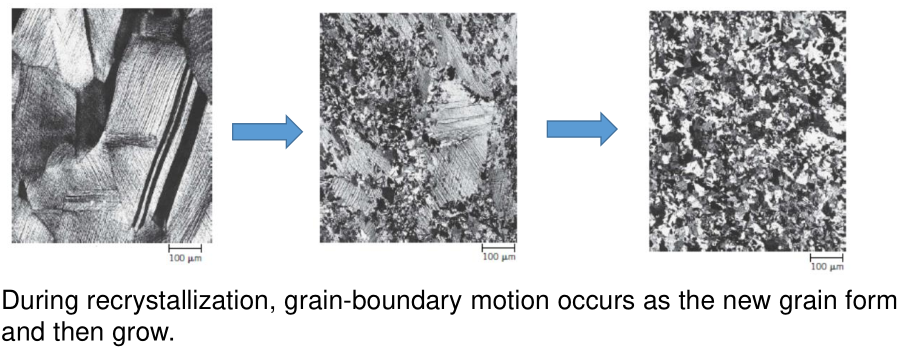
\includegraphics[scale=0.5]{figures/24.png}
\end{center}
\begin{exer}
What is the Recrystallization temperature ?
\end{exer}
temperature at which the process is
complete in one hour. It is typically 1/3 to 1/2 of the melting temperature
(can be as high as 0.7 Tm in some alloys).
\begin{exer}
Discuss grain growth :
\end{exer}
If deformed polycrystalline material is maintained at annealing temperature
following complete recrystallization, then further grain growth occurs.
\begin{center}
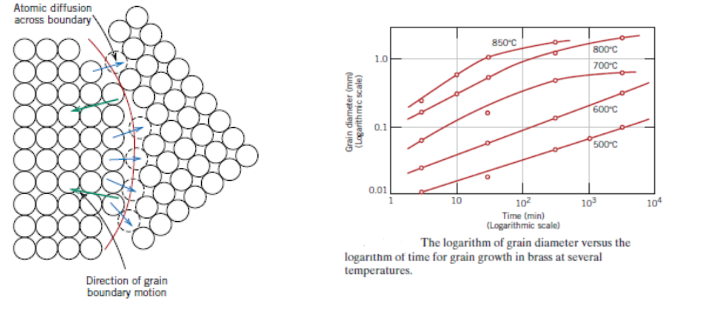
\includegraphics[scale=0.5]{figures/25.png}
\end{center}
\begin{exer}
What is the driving force in grain growth ?
\end{exer}
Driving force is reduction of grain boundary area. Big grains grow at the expense of the small ones.
\begin{exer}
Do grain growth happens only after recrystallization or deformation ?
\end{exer}
No, Grain growth during annealing occurs in all polycrystalline materials (i.e. they do not have to be deformed or recrystallized first). 
\begin{exer}
What causes boundary motion ?
\end{exer}
Boundary motion occurs by diffusion of atoms across the grain boundary.
\begin{center}
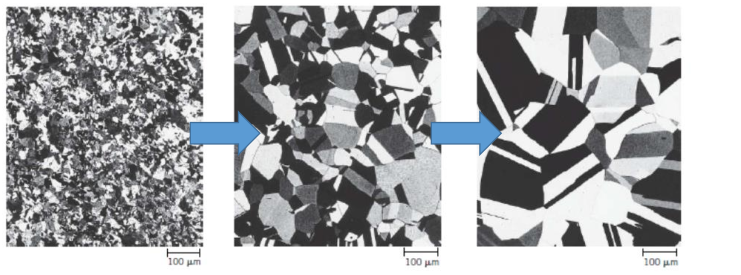
\includegraphics[scale=0.5]{figures/26.png}
\end{center}
\end{document}








